\documentclass[11pt]{article}
\usepackage[margin=1in]{geometry}
\usepackage{amsmath,amssymb}
\usepackage{graphicx}
\usepackage{booktabs}
\usepackage[colorlinks=true,linkcolor=blue,citecolor=blue,urlcolor=blue]{hyperref}

% --- the only two lines to edit before submission ---
\newcommand{\authorname}{Singularity}
\newcommand{\affiliation}{}

\title{Contrastive pretraining on fingerprints improves Tox21 assay\\ ranking for unseen chemical scaffolds}
\author{\authorname\\ \small \affiliation}
\date{\today}

\begin{document}
\maketitle

\begin{abstract}
We test whether contrastive pretraining on molecular fingerprints helps predict Tox21 in-vitro assay labels for
compounds whose chemical scaffolds were absent from training. Two scaffold-grouped splits were fixed in advance,
each with 615 held-out scaffolds. A fingerprint network pretrained to match two randomly masked views of the same
molecule, then fine-tuned on the 12 assays, reached a mean macro average precision of 0.407 in the first split,
against 0.384 for the same network trained from scratch and 0.321 for per-assay logistic regression. Averaging three
initialisations, the contrastive model gained 0.031 over the supervised one (paired scaffold bootstrap 95\% interval
0.008 to 0.052). The second split reproduced the gain: 0.028 (interval 0.012 to 0.040). In both splits the
contrastive ensemble was better on all 12 assays. The cost is about 38 seconds of training instead of 4, and no data
beyond the training compounds is needed.
\end{abstract}

\section{Introduction}
Tox21~\cite{tox21} provides qualitative results of 12 nuclear-receptor and stress-response assays for about 8,000
compounds and is a standard benchmark for molecular property prediction~\cite{moleculenet}. Contrastive
self-supervised learning~\cite{simclr} trains an encoder to give similar representations to two altered views of
the same example. The practical question is whether such pretraining, using only the training compounds and simple
fingerprint-bit masking as the alteration, helps on new chemical series, the setting in which a screening model is
actually used.

\section{Methods}
\paragraph{Data.} The public Tox21 CSV (7,831 records, 12 tasks). Eight SMILES that RDKit could not parse or sanitise
were listed and removed before splitting, leaving 7,823 compounds. Inputs are Morgan fingerprints (radius 2, 1,024
bits). Missing labels stay missing and are masked in training and scoring.
\paragraph{Splits.} Compounds are grouped by Bemis--Murcko scaffold (acyclic compounds get their own key) and each
group is kept in one partition. Split 1 (seeds 2026/2054): 5,955 training, 776 validation and 1,092 test compounds;
split 2 (seeds 2028/2056): 6,179, 707 and 937. An explicit audit confirms that no scaffold crosses partitions in
either split. This is stricter than a random split and not directly comparable with every published benchmark
number.
\paragraph{Models.} Contrastive MLP: two views made by independently hiding 10\% of the fingerprint bits, InfoNCE
loss at temperature 0.20, 80 pretraining epochs on training compounds only; the encoder is then fine-tuned as a
12-task classifier. Supervised MLP: identical architecture and fine-tuning from random initialisation. Logistic
baseline: one class-balanced logistic regression per assay. Neural models use masked binary cross-entropy with
task-specific positive weights, AdamW (learning rate 0.0005), at most 70 epochs, early stopping on validation macro
average precision (patience 10), and seeds 17, 29 and 43. All settings and both splits were written down before the
runs.
\paragraph{Outcome.} Macro average precision (AP) over the 12 assays on the test partition, for individual runs and
for the average of the three probability outputs; paired bootstrap over test scaffolds (1,000 replicates).

\section{Results}
\begin{table}[h]
\centering
\begin{tabular}{lrrrr}
\toprule
 & \multicolumn{2}{c}{split 1} & \multicolumn{2}{c}{split 2} \\
model & macro AP & ensemble AP & macro AP & ensemble AP \\
\midrule
contrastive MLP & \textbf{0.407} $\pm$ 0.004 & \textbf{0.420} & \textbf{0.328} $\pm$ 0.010 & \textbf{0.336} \\
supervised MLP & 0.384 $\pm$ 0.005 & 0.389 & 0.303 $\pm$ 0.014 & 0.308 \\
logistic regression & 0.321 & -- & 0.270 & -- \\
\midrule
ensemble gain [95\% interval] & \multicolumn{2}{r}{+0.031 [0.008, 0.052]} & \multicolumn{2}{r}{+0.028 [0.012, 0.040]} \\
\bottomrule
\end{tabular}
\caption{Held-out scaffolds (615 per split). Macro AP: mean $\pm$ standard deviation over three seeds. Gain:
contrastive minus supervised ensemble, paired scaffold bootstrap.}
\label{tab:results}
\end{table}

\begin{table}[h]
\centering
\begin{tabular}{lrrr|lrrr}
\toprule
assay & contr. & superv. & diff. & assay & contr. & superv. & diff. \\
\midrule
NR-AR & 0.408 & 0.369 & 0.039 & SR-ARE & 0.412 & 0.388 & 0.024 \\
NR-AR-LBD & 0.631 & 0.614 & 0.017 & SR-ATAD5 & 0.296 & 0.293 & 0.002 \\
NR-AhR & 0.614 & 0.582 & 0.032 & SR-HSE & 0.235 & 0.164 & 0.071 \\
NR-Aromatase & 0.281 & 0.225 & 0.056 & SR-MMP & 0.516 & 0.480 & 0.035 \\
NR-ER & 0.521 & 0.493 & 0.028 & SR-p53 & 0.262 & 0.254 & 0.008 \\
NR-ER-LBD & 0.601 & 0.543 & 0.058 & NR-PPAR-$\gamma$ & 0.262 & 0.259 & 0.003 \\
\bottomrule
\end{tabular}
\caption{Ensemble AP by assay in split 1. In split 2 the differences were also positive on all 12 assays (from 0.003
on SR-ARE to 0.058 on NR-ER-LBD).}
\label{tab:assays}
\end{table}

\begin{figure}[h]
\centering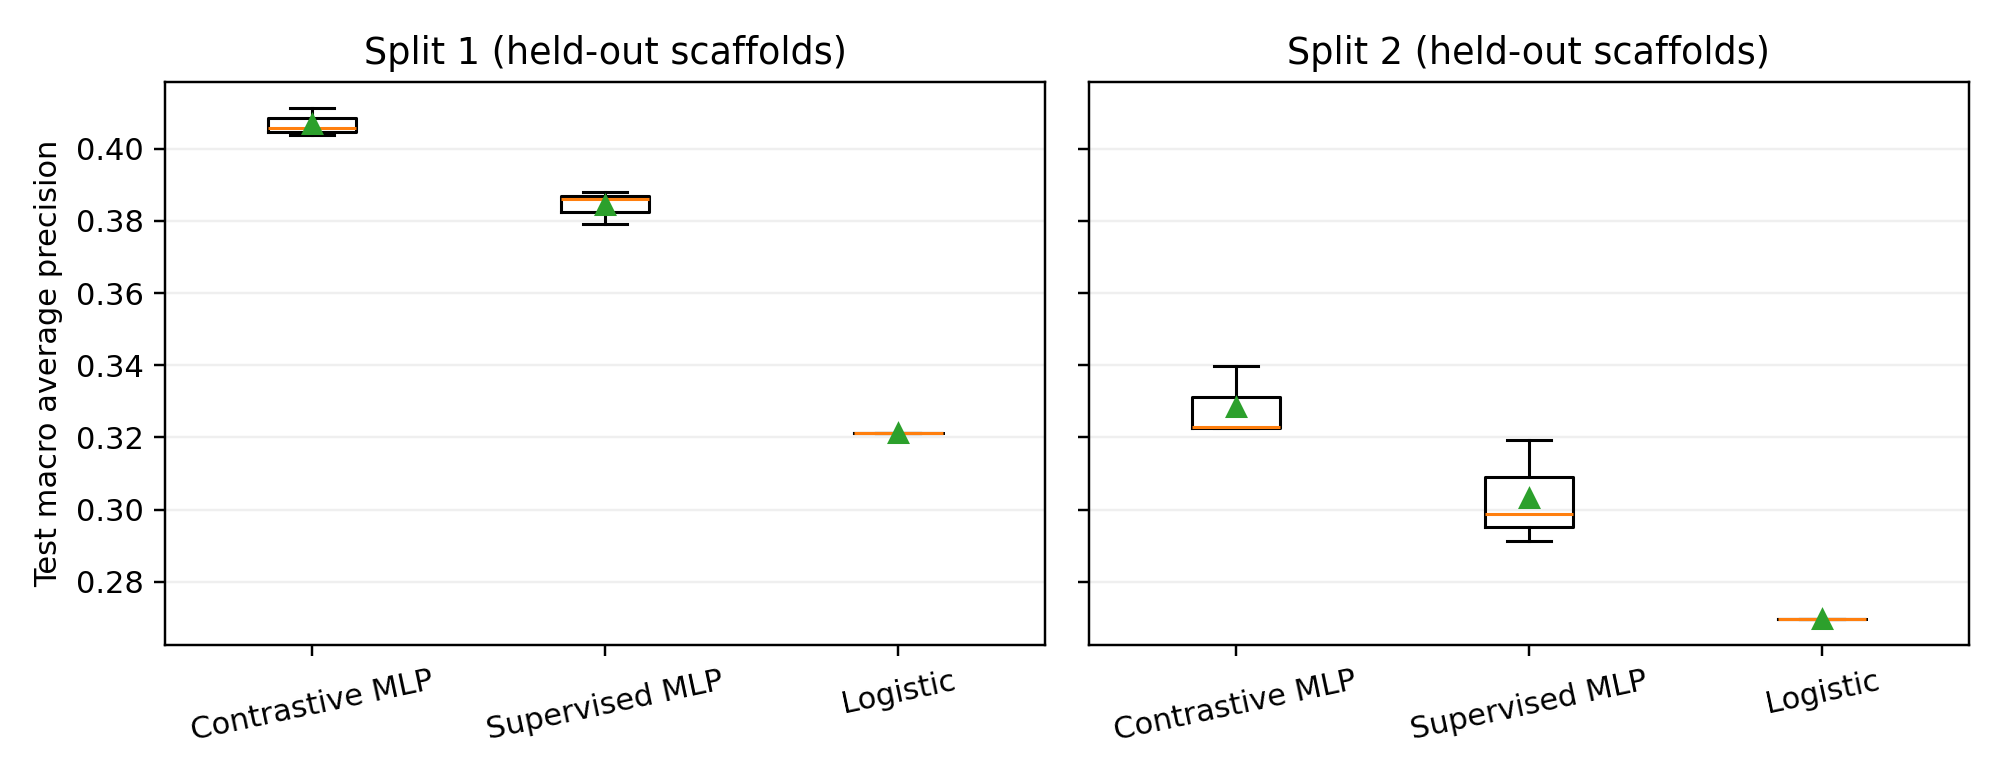
\includegraphics[width=\linewidth]{fig_results.png}
\caption{Test macro average precision per seed in the two scaffold splits; triangles mark the mean.}
\label{fig:results}
\end{figure}

\begin{itemize}
\item \textbf{Consistent gain.} Contrastive pretraining beat training from scratch in both splits, by 0.031 and
0.028 in ensemble AP, with paired intervals above zero (Table~\ref{tab:results}).
\item \textbf{Broad, not one assay.} The ensemble gain was positive on all 12 assays in both splits; the largest were
on SR-HSE, NR-ER-LBD and NR-Aromatase (Table~\ref{tab:assays}).
\item \textbf{Ranking also improves.} Macro ROC-AUC rose from 0.761 to 0.778 (split 1) and from 0.734 to 0.743
(split 2).
\item \textbf{Cost.} About 38--40 seconds per contrastive run including pretraining, against about 4 seconds.
\end{itemize}

\section{Discussion}
Even with the simplest possible augmentation, masking fingerprint bits, and no extra unlabelled molecules, contrastive
pretraining gave a representation that transferred better to unseen scaffolds than direct supervised training of the
same network. Because pretraining used only the training compounds, the gain comes from the objective rather than
from more data, which suggests that larger unlabelled libraries and chemistry-aware augmentations could add further.

\paragraph{Limitations.} One dataset and two scaffold splits; Tox21 labels are in-vitro assay outcomes. The models,
splits and metric were fixed in advance, but not a numerical success threshold. Graph-based and large pretrained
models were not compared.

\paragraph{Reproducibility.} \texttt{experiment.py} runs both splits, the scaffold audit and the consolidation in
order. \texttt{results.json} contains the combined audit, per-seed and ensemble metrics, per-assay differences and
the bootstrap for both splits; per-compound test predictions are in \texttt{code/}.

\paragraph{Origin of the question.} The question came from an automated forecast (Singularity v3, registered on 5
November 2026 with a SHA-256 fingerprint, view without generative AI) that contrastive learning would enter the
subfield \emph{Health, Toxicology and Mutagenesis}. The forecast concerned the arrival of the method, not the result
of this study.

\begin{thebibliography}{9}
\bibitem{tox21} R.~Huang et al., Tox21 Challenge to build predictive models of nuclear receptor and stress response
pathways as mediated by exposure to environmental chemicals and drugs, \emph{Frontiers in Environmental Science} 3, 85
(2016).
\bibitem{moleculenet} Z.~Wu et al., MoleculeNet: a benchmark for molecular machine learning, \emph{Chemical Science}
9, 513--530 (2018).
\bibitem{simclr} T.~Chen, S.~Kornblith, M.~Norouzi and G.~Hinton, A simple framework for contrastive learning of
visual representations, \emph{ICML} (2020).
\end{thebibliography}
\end{document}
